\documentclass[10pt]{article}
\usepackage[margin=0.85in]{geometry}
\usepackage{amsmath,amssymb}
\usepackage[T1]{fontenc}
\usepackage[utf8]{inputenc}
\usepackage{lmodern}
\usepackage{microtype}
\usepackage{enumitem}
\usepackage{booktabs}
\usepackage{graphicx}
\usepackage{url}
\usepackage[hidelinks]{hyperref}
\hypersetup{pdftitle={No External-Field Effect: Cluster-Satellite Lensing, the Cassini Quadrupole and the Outer Solar System Point to an EFE-Blind MOND Sector}, pdfauthor={The authors}}
\setlist{nosep,leftmargin=1.3em}
\setlength{\parskip}{3pt}\setlength{\parindent}{0pt}
\sloppy
\newcommand{\fpath}[1]{\nolinkurl{#1}}
\begin{document}

\begin{center}
{\Large\bfseries No External-Field Effect:\\ Cluster-Satellite Lensing, the Cassini Quadrupole and the Outer Solar System\\ Point to an EFE-Blind MOND Sector}\\[6pt]
{\small The authors --- 2026-10-08, version 1.1 (corrections; v1.0: doi:10.5281/zenodo.23196661) --- AI-assisted research programme; not peer reviewed}
\end{center}

% Every number below is parsed from committed outputs by make_paper44_figures.py (PAPER44_figures_numbers.json) and checked by PAPER44_audit.py.
% Lanes: sonnet55_push/cold_mass/cm08, cm14b, cm15; sonnet55_push/puzzle_32pi/p57, p58.

\begin{abstract}
\noindent In modified-gravity versions of MOND a system's internal boost depends on the external gravitational field it sits in (the external-field effect, EFE). We test the quadrature law $g^2=g_N^2+a_0g_N$ with $a_0=\tfrac12c\sqrt{G\rho_\Lambda}$ against three data sets that are sensitive to the EFE in different ways. (i) Weak lensing of satellite galaxies in massive clusters (Sif\'on et al.\ 2018, five stellar-mass bins) is fitted by the full, isolated boost with $\chi^2=0.7$ for 5 bins and a mean offset of $+0.01$\,dex; the same law with the cluster's field included, $\eta=g_{\rm ext}/a_0=0.59$--$0.81$, fails by $\chi^2=99.7$, and a direction-blind rule that keeps only the field's magnitude fails equally ($\chi^2=99.5$). (ii) The anisotropic part of the EFE predicts a Cassini quadrupole $Q_2=2.195\times10^{-26}$\,s$^{-2}$, $6.3\sigma$ above the measured value. (iii) In the outer Solar System the Galactic EFE pumps the perihelia of detached trans-Neptunian objects, while a central force conserves them; the pre-registered verdict of that secular run was inconclusive. The data therefore ask for a MOND sector whose boost is computed from a bound system's own field alone. This costs two results that preferred an EFE, the Milky Way's Gaia DR3 outer decline and Chae's rotation-curve signal, and it makes a sharp prediction for Gaia DR4: wide binaries boosted as isolated MOND systems, $\gamma_v=\sqrt{\nu}\approx1.20$ at 10\,kAU and $1.51$ at 20\,kAU for $1.5\,M_\odot$. No covariant theory with this property exists yet.
\end{abstract}
% AUDIT: E01

\section{Cluster-satellite lensing}
Sif\'on et al.\ (2018) measured subhalo masses $m_{\rm bg}$ of satellites in MENeaCS clusters ($z<0.15$; median dynamical host mass $M_{200}\sim6\times10^{14}M_\odot$) inside $r_{\rm bg}$, where the subhalo density equals the host's local density. We read their table directly (five bins, $\log M_*=9.51$--$11.01$) and estimate $r_{\rm bg}=36$--$149$\,kpc by matching an isothermal subhalo to an NFW host ($M_{200}=6\times10^{14}M_\odot$, $c=4$). Each satellite's baryons are $1.2\,M_*$; we add the galaxy-level retained cold mass found in early-type galaxies (13\% of the cosmic share), which contributes about 5\%. At $r_{\rm bg}$ the internal field is tiny, $x=g_N/a_0=0.004$--$0.008$, while the cluster's field is $\eta=0.59$--$0.81$.
\begin{center}
\begin{tabular}{lcc}
\toprule
reading & $\chi^2$ (5 bins) & mean offset (dex)\\
\midrule
isolated boost $\nu(x)$ (no EFE) & 0.7 & $+0.01$\\
magnitude EFE $\nu(\sqrt{x^2+\eta^2})$ & 99.5 & --\\
linear EFE $\nu(x+\eta)$ & 99.7 & $+0.81$\\
no phantom in a bound satellite (``ownership'') & 131.6 & $+0.93$\\
\bottomrule
\end{tabular}
\end{center}
% AUDIT: E02
Any rule that lets the cluster's field enter the satellite's boost caps $\nu$ near 1.5 instead of 11--15. $\Lambda$CDM also fits these data (it is the paper's model), so this test separates readings of MOND, not MOND from $\Lambda$CDM.
\begin{figure}[h]\centering
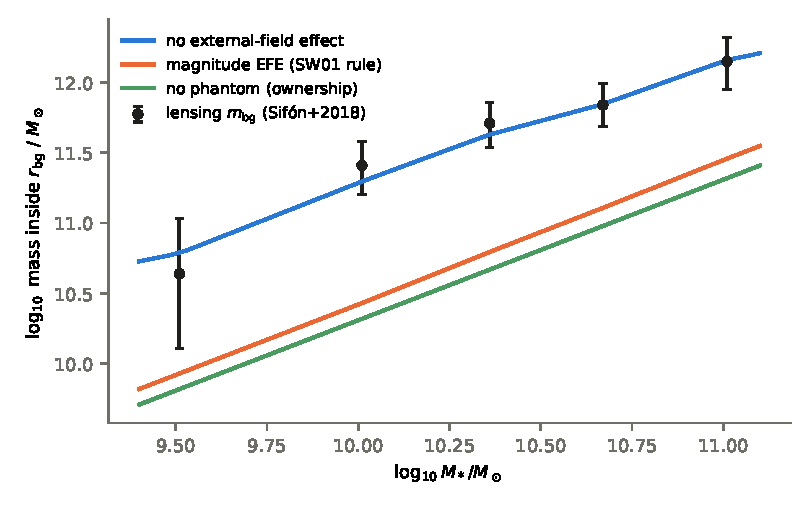
\includegraphics[width=0.72\textwidth]{fig1_paper44_satellites.pdf}
\caption{Satellite masses inside $r_{\rm bg}$ (points) against three readings of the law.}\label{fig:sat}
\end{figure}

\section{The Cassini quadrupole and the outer Solar System}
Solving the QUMOND field equation for the Sun in the Galactic field (multipole solver, observed $g_{\rm ext}=2.146\times10^{-10}$\,m\,s$^{-2}$) gives $Q_2=2.195\times10^{-26}$\,s$^{-2}$, $6.3\sigma$ above Cassini's $(3\pm3)\times10^{-27}$ (Hees et al.\ 2014); Cassini alone would require $\kappa<0.171$ ($2\sigma$). With the EFE removed $Q_2=0$. In a secular model of detached trans-Neptunian objects (giant-planet quadrupole, Galactic tide, the QUMOND anomaly), the EFE's quadrupole drives large perihelion changes. With the EFE, 57\% of objects are driven below $q=25$\,AU and the detached occupancy is 0.195, against 19\% and 0.067 for Newton. A control run with only the central monopole (planets and tide off) conserves perihelia to 0.005\,AU over 200\,Myr, as a central force must. That run's pre-registered verdict was inconclusive: the numbers are small and Neptune scattering is not modelled. The EFE is what makes MOND overpopulate the detached disc (Vokrouhlick\'y, Nesvorn\'y \& Tremaine 2024).
% AUDIT: E03

\section{What an EFE-free rule costs and predicts}
Two results in this programme preferred an EFE: the Milky Way's Gaia DR3 outer decline and Chae's rotation-curve EFE signal. For the first, the isolated kernel ($\nu_{\rm RAR}$ in that lane) is $2.3$--$2.4\sigma$ too shallow nominally and up to $2.5\sigma$ for the least favourable (shallowest) baryonic model. A 1-D LMC field model reduces this to 1.1--1.6$\sigma$, and disequilibrium is not modelled. For the second, refitted with this law, it is $1.7\sigma$ on the canonical footing and $2.7\sigma$ on the alternative ($2.2$ and $3.0\sigma$ with $\nu_{\rm mono}$). WALLABY cannot decide: its directional-EFE stack gives an amplitude of $-1.70$ on a scale where AQUAL is $+1$, with error $\pm2.98$ (analytic; $\pm2.12$ bootstrap), i.e.\ $0.6\sigma$ from zero and $0.9\sigma$ from AQUAL; the run is consistent with AQUAL and with no EFE alike. An EFE-free rule gives up both. In exchange it predicts wide binaries boosted as isolated systems: $\gamma_v=\sqrt{\nu(y)}=1.06$, $1.20$, $1.51$ at 5, 10, 20\,kAU for $1.5\,M_\odot$ (3-D separation; the registered statistic is not recomputed here), against $1.11$ at 20\,kAU for the magnitude rule and 1 for Newton (Fig.~\ref{fig:wb}). Gaia DR4 (December 2026) decides; a Newtonian result would exclude this reading.
% AUDIT: E04
\begin{figure}[h]\centering
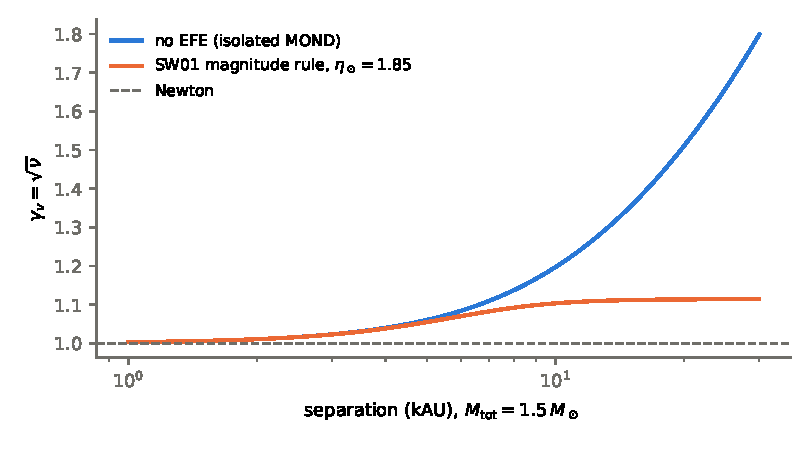
\includegraphics[width=0.72\textwidth]{fig2_paper44_widebinaries.pdf}
\caption{Wide-binary velocity boost for the EFE-free rule, the magnitude-only rule and Newton.}\label{fig:wb}
\end{figure}

\section{Summary}
Satellite lensing, the Cassini quadrupole and the outer Solar System each disfavour an external-field effect, the first even in its direction-blind, magnitude-only form. The consistent reading is a MOND sector computed from each bound system's own field. No covariant action with this property is known; the programme's direction-blind construction keeps the field's magnitude and is excluded by the satellites. The test is Gaia DR4. The coefficient $\kappa=\tfrac12$ remains fitted; the cold mass of cosmology is still required.

\paragraph{Reproducibility.} \fpath{sonnet55_push/cold_mass/cm14b_sifon_table.py}, \fpath{cm15_sw01_rule_vs_satellites.py}, \fpath{cm08_etg_retained_fraction.py}; \fpath{sonnet55_push/puzzle_32pi/p58_cassini_kappa_bound.py}, \fpath{p57_etno_secular_nbody.py}, \fpath{qumond_efe_multipole.py}; fetch log \fpath{data_assembly/sifon2018/}; figures \fpath{make_paper44_figures.py}; audit \fpath{PAPER44_audit.py}.

\small
\paragraph{References.}
Sif\'on C. et al., MNRAS 478, 1244 (2018), arXiv:1706.06125.
Hees A., Folkner W. M., Jacobson R. A., Park R. S., Phys.\ Rev.\ D 89, 102002 (2014).
Vokrouhlick\'y D., Nesvorn\'y D., Tremaine S., ApJ 968 (2024), arXiv:2403.09555.
Milgrom M., Phys.\ Lett.\ A 253, 273 (1999).
\end{document}
